%===================================================================================
% Chapter: Metodologia
%===================================================================================
\chapter{Metodología}\label{chapter:metodologia}
%\addcontentsline{toc}{chapter}{Marco Teórico}
%===================================================================================

En este capítulo se describe la metodología y la estructura empleada en la implementación de una simulación computacional del sistema inmune de un lactante, integrando conceptos de inmunología computacional y sistemas complejos para modelar la respuesta a vacunas conjugadas neumocócicas.

El simulador se estructura en dos capas principales:
\begin{enumerate}
    \item Modelado de agentes biológicos:
        \begin{enumerate}
            \item Antígenos
            \item Células B
        \end{enumerate}
    \item Entornos de Interacción:
        \begin{enumerate}
            \item Centros germinales
            \item Sistema inmune
        \end{enumerate}
\end{enumerate}
\section{Modelado de agentes biológicos}
\begin{enumerate}
    
    \item \texttt{Antígeno}: Representado por un vector de epítopos, cantidad de polisacárido, proteína portadora y factor de inmunogenicidad.
    \item \texttt{Célula B}: 
    Representada por un identificador, un vector de receptores, un serotipo asociado que representa el antígeno que ha reconocido y una afinidad por este.
\end{enumerate}

    


\section{Centros Germinales}

Los centros germinales constituyen conglomerados de células B que reconocen el mismo antígeno en los cuales estas se dividen rápidamente.
\subsection{Procesos Inmunológicos clave}
En los centros germinales ocurren procesos en función de la especialización y diferenciación de las células B.
\begin{enumerate}
    \item \textbf{Cálculo de afinidad:}
     
    La afinidad entre una célula B y un antígeno se calcula mediante la distancia euclidiana entre sus vectores característicos:

    $$
    A = e^{-||\vec{r}_{B} - \vec{e}_{A}||}
    $$
    
    donde:
    
        
    - $\vec{r}_B$ es el vector de receptores de la célula B.
        
    - $\vec{e}_A$ es el vector de epítopos del antígeno.
        
    - $A$ representa la afinidad (valor entre 0 y 1).
    \item \textbf{Selección:}
    
    La selección de células B se realiza mediante un algoritmo tipo Boltzmann, que pondera probabilísticamente la supervivencia según su afinidad. Este proceso permite explorar soluciones subóptimas manteniendo diversidad genética.
    \item \textbf{Diferenciación:}
    
    Según su afinidad, las células B pueden diferenciarse en:
        \begin{enumerate}
            \item Células de memoria 
            \item Células plasmáticas 
        \end{enumerate}
    \item \textbf{Mutación:}
    
    Las células B pueden mutar sus receptores con cierta probabilidad (\texttt{mutation\_p}), aplicando variaciones gaussianas limitadas a cada componente del vector receptor. Esta mutación ocurre tanto dentro de los centros germinales como en el sistema inmune global.
\end{enumerate}

\begin{figure}[H] % h = here (aquí)
    \centering
    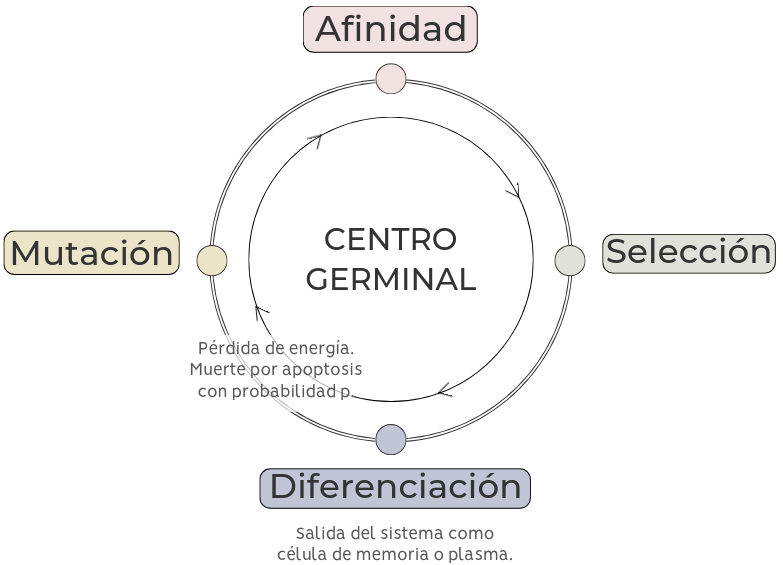
\includegraphics[width=1\textwidth]{Graphics/gc.png}
    \caption{Ciclo que ocurre dentro del Centro Germinal}
    \label{fig:cg}
\end{figure}

Las células B entran al centro germinal una vez calculada su afinidad con el antígeno, mediante el proceso de selección se eligen las células que son candidatas a salir del centro germinal y son clasificadas por el proceso de selección como células de memoria o plasma y enviadas de vuelta al sistema inmune. Las células restantes pueden morir por pérdida de energía (apoptosis) o sobrevivir, dividirse y mutar. Posteriormente se recalcula su afinidad con el antígeno y el ciclo se repite hasta que mueren todas las células del centro germinal.

\section{Sistema Inmune}

El sistema inmune consta de un grupo de células B \textit{naive} que se dividen y mutan o mueren. Ante la presencia de antígeno (vacunación) estas células pueden pasar a formar parte de centros germinales. 

Los centros germinales una vez terminan cada ciclo devuelven al sistema inmune las células que han evolucionado a células de memoria o plasma y estas son utilizadas para medir la concentración de anticuerpos que se utiliza para medir la respuesta inmune del sujeto.

Las células que no pasan a formar parte de los centros germinales continúan en el mismo ciclo que se encontraban antes de la presencia del antígeno.

\begin{figure}[H] % h = here (aquí)
    \centering
    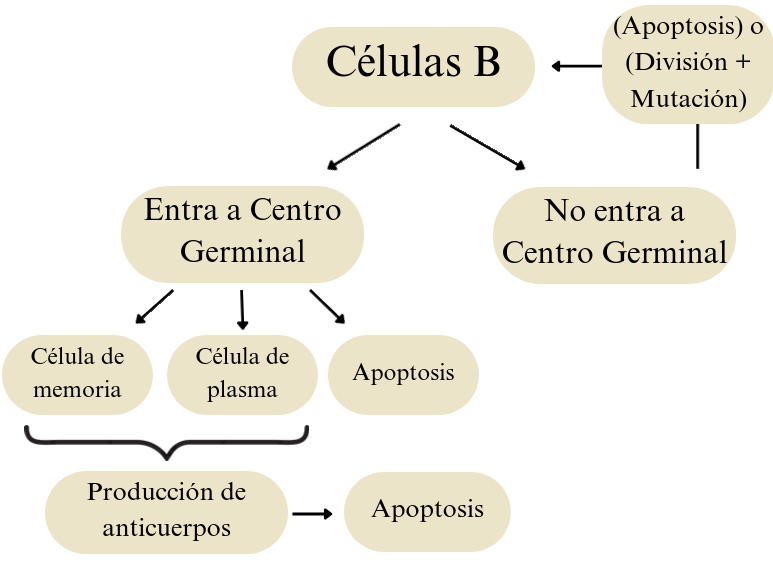
\includegraphics[width=1\textwidth]{Graphics/is.png}
    \caption{Células B dentro del sistema inmune}
    \label{fig:is}
\end{figure}




% aaaaaaaaaaaaaaaaaaaaaaaaaaaaaaaaaaaaaaaaaaaaaaaaaaaaaaaaaaaaaaaaaaaaaaaaaaaaaaaaaaa
% aaaaaaaaaaaaaaaaaaaaaaaaaaaaaaaaaaaaaaaaaaaaaaaaaaaaaaaaaaaaaaaaaaaaaaaaaaaaaaaaaaa
% aaaaaaaaaaaaaaaaaaaaaaaaaaaaaaaaaaaaaaaaaaaaaaaaaaaaaaaaaaaaaaaaaaaaaaaaaaaaaaaaaaa
% aaaaaaaaaaaaaaaaaaaaaaaaaaaaaaaaaaaaaaaaaaaaaaaaaaaaaaaaaaaaaaaaaaaaaaaaaaaaaaaaaaa
% aaaaaaaaaaaaaaaaaaaaaaaaaaaaaaaaaaaaaaaaaaaaaaaaaaaaaaaaaaaaaaaaaaaaaaaaaaaaaaaaaaa


